%Option twoside zur Optimierung für beidseitigen Druck
\documentclass[12pt,ngerman,numbers=noenddot,abstract=true,version=first,headsepline]{scrreprt}
\renewcommand{\familydefault}{\sfdefault}
\usepackage[T1]{fontenc}
\usepackage[utf8]{inputenc}
\usepackage{geometry}
\geometry{verbose,tmargin=2.5cm,bmargin=2.5cm,head=35pt}
\setlength{\parskip}{\medskipamount}
\setlength{\parindent}{0pt}
\usepackage{array}
\usepackage{float}
\usepackage{textcomp}
\usepackage{multirow}
\usepackage{amsmath}
\usepackage{amsthm}
\usepackage{graphicx}
\usepackage{setspace}
\usepackage{microtype}
\usepackage{nomencl}
\usepackage{wrapfig}
\usepackage[style=super, nopostdot, nonumberlist, nogroupskip, acronyms]{glossaries}

\def\changemargin#1#2{\list{}{\rightmargin#2\leftmargin#1}\item[]}
\let\endchangemargin=\endlist

\setstretch{1.2}

\makeatletter

% verschieden Symbole, Zeichen wie (c), €
\usepackage{textcomp,units}

% Mehr Platz zwischen Tabelle und Untertitel
\usepackage{caption}
\captionsetup[table]{skip=10pt}

%Kapitelzahl sehr groß
\makeatletter% siehe De-TeX-FAQ 
    \renewcommand*{\chapterformat}{% 
    \begingroup% damit \unitlength-Änderung lokal bleibt 
    \setlength{\unitlength}{1mm}% 
    \begin{picture}(10,10)(0,5) 
        \setlength{\fboxsep}{0pt} 
        %\put(0,0){\framebox(20,40){}}% 
        %\put(0,20){\makebox(20,20){\rule{20\unitlength}{20\unitlength}}}% 
        \put(10,15){\line(1,0){\dimexpr 
            \textwidth-20\unitlength\relax\@gobble}}% 
        \put(0,0){\makebox(10,20)[r]{% 
            \fontsize{28\unitlength}{28\unitlength}\selectfont\thechapter 
            \kern-.05em% Ziffer in der Zeichenzelle nach rechts schieben 
            }}% 
        \put(10,15){\makebox(\dimexpr 
            \textwidth-20\unitlength\relax\@gobble,\ht\strutbox\@gobble)[l]{% 
            \ \normalsize\color{black}\chapapp~\thechapter\autodot 
            }}% 
        \end{picture} % <-- Leerzeichen ist hier beabsichtigt! 
    \endgroup 
}

\usepackage{ %a4wide,
            ellipsis, mparhack, %Fehlerkorrektur für Marginalien
            booktabs, longtable %schönere Tabellen
}


%Kurzfassung und Abstract (englisch) auf eine Seite
\renewenvironment{abstract}{
    \@beginparpenalty\@lowpenalty
    \begin{center}
    \normalfont\sectfont\nobreak\abstractname
    \@endparpenalty\@M
    \end{center}
}{
    \par
}

% schönerer Blocksatz!!
\usepackage{ifpdf} % part of the hyperref bundle
\ifpdf % if pdflatex is used 

%set fonts for nicer pdf view
\IfFileExists{lmodern.sty}{\usepackage{lmodern}}
    {\usepackage[scaled=0.92]{helvet}
    \usepackage{mathptmx}
    \usepackage{courier} }
\fi

% the pages of the TOC are numbered roman
% and a pdf-bookmark for the TOC is added
\pagenumbering{roman}
\let\myTOC\tableofcontents
\renewcommand\tableofcontents{
%\pdfbookmark[1]{Contents}{}
\myTOC
\clearpage
\pagenumbering{arabic}}

%Bezeichungen anpassen
%Babelpaket muß zuvor geladen werden
\usepackage[ngerman]{babel}
\addto\captionsngerman{ 
    \renewcommand{\figurename}{Abb.}% 
    \renewcommand{\tablename}{Tab.}% 
    \renewcommand{\abstractname}{Kurzfassung}
    \renewcommand{\nomname}{Abkürzungsverzeichnis}
}

%mehr Platz zwischen Überschrift und Tabelle
\newcommand{\@ldtable}{}
    \let\@ldtable\table
\renewcommand{\table}{ %
    \setlength{\@tempdima}{\abovecaptionskip} %
    \setlength{\abovecaptionskip}{\belowcaptionskip} %
    \setlength{\belowcaptionskip}{\@tempdima} %
    \@ldtable}

%Config für Programmcode
\usepackage{listings}
\usepackage{color}
\usepackage{scrhack}

\renewcommand{\lstlistlistingname}{Programm-Listings}

\definecolor{dkgreen}{rgb}{0,0.6,0}
\definecolor{gray}{rgb}{0.5,0.5,0.5}
\definecolor{mauve}{rgb}{0.58,0,0.82}

\lstset{frame=tb,
    language=Java,
    aboveskip=3mm,
    belowskip=3mm,
    showstringspaces=false,
    columns=flexible,
    basicstyle={\footnotesize\ttfamily},
    numbers=left,
    numberstyle=\tiny\color{gray},
    keywordstyle=\color{blue},
    commentstyle=\color{dkgreen},
    stringstyle=\color{mauve},
    breaklines=true,
    breakatwhitespace=true,
    tabsize=3
}

\AtBeginDocument{
    \def\labelitemiii{\(\circ\)}
}


\renewcommand{\author}{"Geogram" - Benita Dietrich, Paul Finkbeiner, Josua Stricker, Jonas Schwarz, Sven Stoll und Moris Kotsch}
\renewcommand{\title}{Geogram - Dokumentation}
\renewcommand{\subject}{Thema}
\newcommand{\keywords}{}

\usepackage[automark,autooneside=false]{scrlayer-scrpage}
\clearscrheadfoot
\if@twoside
    \ofoot[\pagemark]{\pagemark}
    \ohead{\headmark}
\else
    \cfoot[\pagemark]{\pagemark}
    \ohead{
        \ifnum\value{section}>0
        \rightmark
        \fi
    }
    \ihead{
        \leftmark
    }
\fi

\makeatother

% Alle Querverweise und URLs als Link darstellen
% In der PDF-Ausgabe
\usepackage[colorlinks=true, bookmarks, bookmarksnumbered, bookmarksopen, bookmarksopenlevel=1,
    linkcolor=black, citecolor=black, urlcolor=blue, filecolor=blue,
    pdfpagelayout=OneColumn, pdfnewwindow=true,
    pdfstartview=XYZ, plainpages=false, pdfpagelabels,
    pdfauthor={\author{}}, pdftex,
    pdftitle={\title{}},
    pdfsubject={\subject{}},
    pdfkeywords={\keywords{}}]{hyperref}

\usepackage{babel}
\begin{document}
    \pagestyle{plain}
    \titlepage
\begin{center}
    \textbf{\large{}Duale Hochschule Baden-Württemberg }{\large\par}
    \par
\end{center}
\begin{center}
    \textbf{\large{}Stuttgart Campus Horb}{\large\par}
    \par
\end{center}
\begin{center}
    \begin{tabular}{l||r}
        \multicolumn{2}{c}{\vspace{1cm}}
        \tabularnewline
        \multicolumn{2}{c}{
\includegraphics[height=3.5cm]{images/dhbwlogo}}
        \tabularnewline
        \multicolumn{2}{c}{}
        \tabularnewline
        \multicolumn{2}{c}{
\includegraphics[width=0.3\textwidth, scale=1]{images/logo.png}}
        \tabularnewline
        %\multicolumn{2}{c}{\vspace{0.5cm}}
        %\tabularnewline
    \end{tabular}
    \par
\end{center}
\vspace{0.5cm}

\begin{flushleft}
    \textbf{\Large{}\title{}}{\Large\par}
    \par
\end{flushleft}

\begin{flushleft}
    \textbf{\textit{T3INF4310 - Entwicklung mobiler Applikationen}}
    \par
\end{flushleft}

\begin{flushleft}
    {\Large{}\rule[0.5ex]{1\columnwidth}{1pt}}{\Large\par}
    \par
\end{flushleft}

\begin{tabular}{ll}
    eingereicht von:\hspace{1cm} & Benita Dietrich, Paul Finkbeiner, Josua Stricker,
    \tabularnewline
    & Jonas Schwarz, Sven Stoll und Moris Kotsch
    \tabularnewline
    Modul: & T3INF4310 - Entwicklung mobiler Applikationen
    \tabularnewline
    Dozent: & B.Sc. Torsten Hopf
    \tabularnewline
    Kurs: & TINF2018
    \tabularnewline
    Studiengang: & Informatik
    \tabularnewline
    Hochschule: & DHBW Stuttgart Campus Horb
    \tabularnewline
    Bearbeitungszeitraum: & 21.12.2020 - 08.03.2021
    \tabularnewline
    \tabularnewline
    \multicolumn{2}{l}{Horb am Neckar, \today}
    \tabularnewline
\end{tabular}

\begin{flushleft}
    \newpage{}
    \par
\end{flushleft}
    \newpage

    \tableofcontents
    \newpage

    \pagenumbering{roman}
    %ACHTUNG: Korrekte Seitenzahl bei Fertigstellung des Dokuments einstellen, andernfalls ist die Nummerierung u.U. fehlerhaft.
    \setcounter{page}{7}

    \listoffigures
    \newpage

    %\lstlistoflistings
    %\newpage

    %\listoftables
    %\newpage

    %asd
    %GGF anpassen
    %Index aktualisieren mit: makeindex Vorlage.nlo -s nomencl.ist -o Vorlage.nls
    %\printnomenclature[3cm]{}
    %\newpage

    \pagenumbering{arabic}
    %Kopfzeile aktivieren
    \pagestyle{headings}

    \input{chapters/1-Einführung.tex}
\chapter{Konzeption\label{chap2:Zweites-Kapitel}}

Während der Konzeptionsphase ging es darum einen ersten Entwurf für die spätere Implementierung zu entwerfen. Hierfür wurden verschiedene Mockups erstellt, welche einen ersten Einblick in die Designvorstellungen für die mobile Anwendung \glqq Geogram\grqq{} geben sollen.

Mit dem Definieren der MVP-Kriterien, wurde der Funktionsumfang, für die erste minimal funktionsfähige Iteration der mobile Anwendung \glqq Geogram\grqq{} aufgelistet. Zusätzlich wurden noch weitere Soll- und Kann-Kriterien festgelegt.

\section{Mockup's\label{sec2.1:Unterpunkt-1}}

In \autoref{fig:login_white} und \autoref{fig:login_black} ist die Login-Ansicht abgebildet. Bereits als Mockup realisiert, ist der Wechsel zwischen einem White- und Dark-Mode der mobilen Anwendung.

\begin{figure}[H]
    \centering
    \begin{minipage}{.5\textwidth}
      \centering
      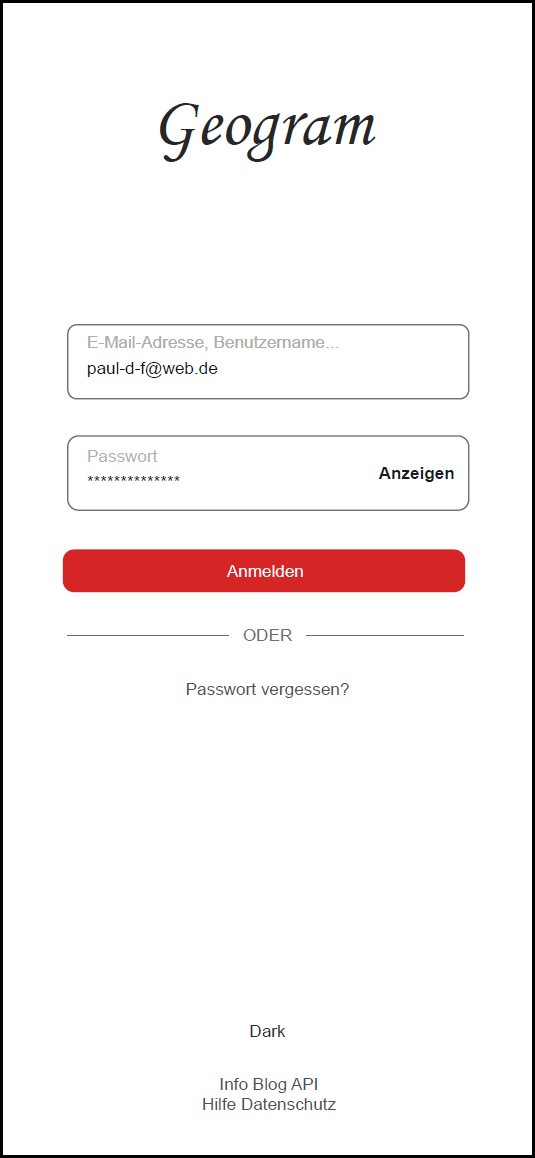
\includegraphics[width=.6\linewidth]{images/Login_MockUp.png}
      \caption{Login-Ansicht in weiß}
      \label{fig:login_white}
    \end{minipage}%
    \begin{minipage}{.5\textwidth}
      \centering
      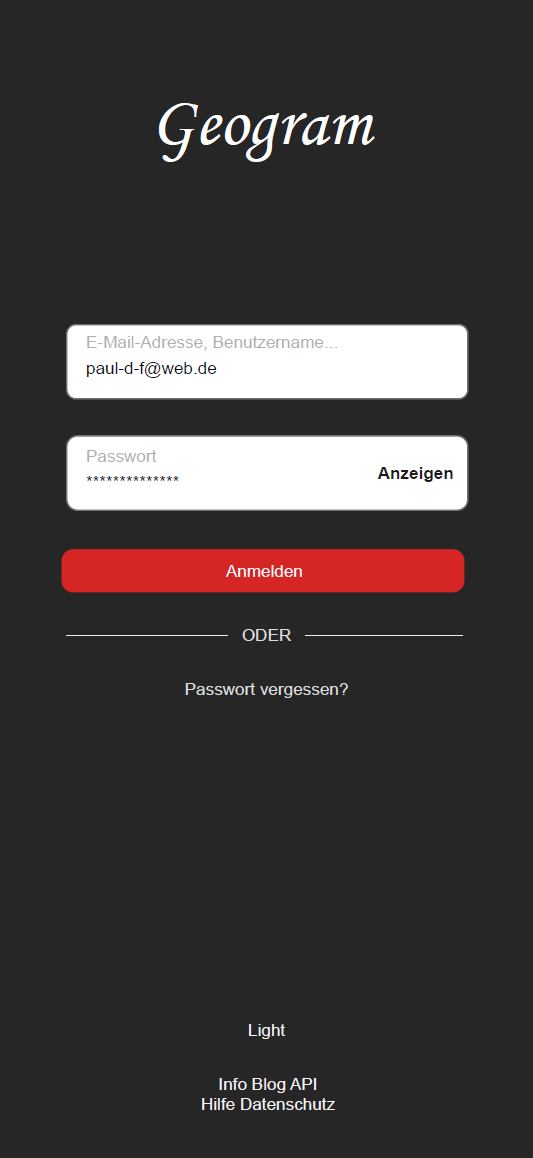
\includegraphics[width=.6\linewidth]{images/Login_MockUp_Black.png}
      \caption{Login-Ansicht in schwarz}
      \label{fig:login_black}
    \end{minipage}
\end{figure}

In \autoref{fig:feed_overview} und \autoref{fig:feed_detail} sind die Feed-Ansichten abgebildet. Die Feed-Übersicht ähnelt der Feed-Übersicht von Instagram, jedoch mit dem Unterschied, dass mithilfe einer Standortangabe die Filterung der Feeds vollzogen wird.

\begin{figure}[H]
    \centering
    \begin{minipage}{.5\textwidth}
        \centering
        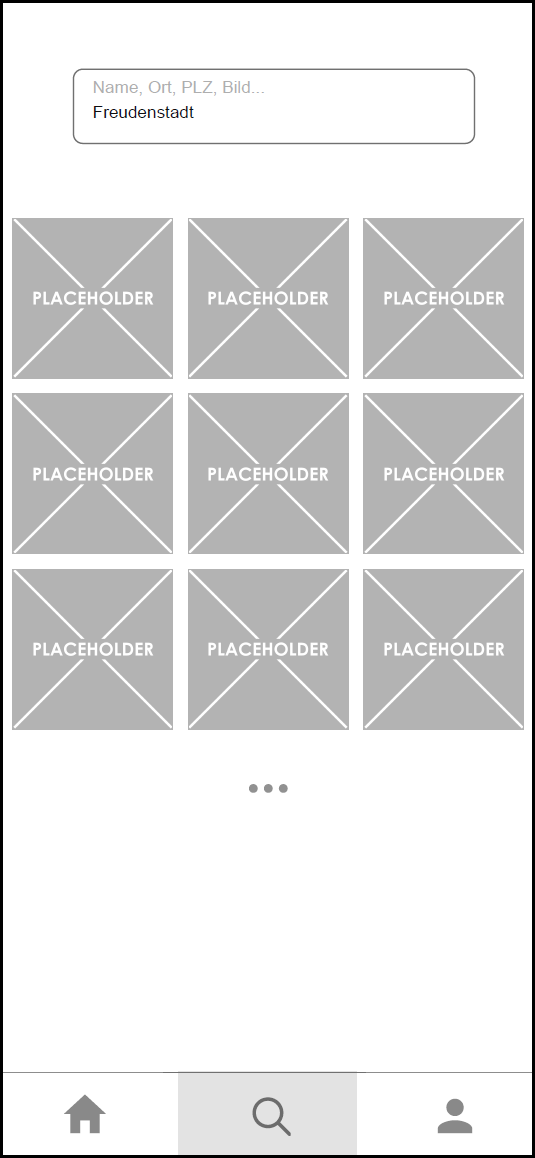
\includegraphics[width=.6\linewidth]{images/Feed_Overview_MockUp.png}
        \caption{Feed Overview}
        \label{fig:feed_overview}
    \end{minipage}%
    \begin{minipage}{.5\textwidth}
      \centering
      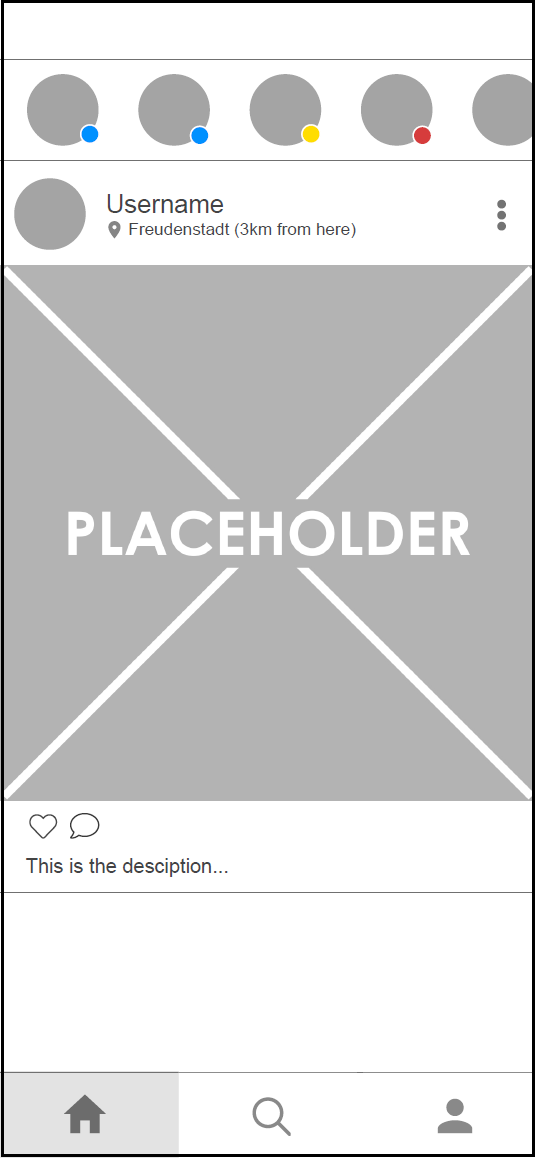
\includegraphics[width=.6\linewidth]{images/Feed_Detail_MockUp.png}
      \caption{Feed Detail}
      \label{fig:feed_detail}
    \end{minipage}
\end{figure}

Die folgenden zwei Abbildungen zeigen die Profilansicht mit Änderungsmöglichkeit.

\begin{figure}[H]
    \centering
    \begin{minipage}{.5\textwidth}
      \centering
      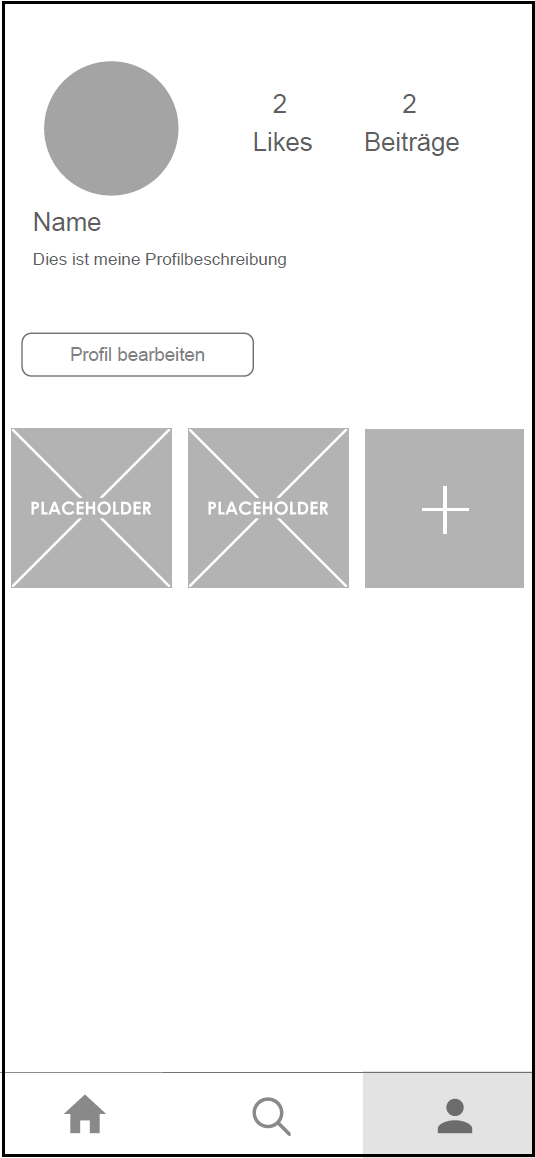
\includegraphics[width=.6\linewidth]{images/Profil_MockUp.png}
      \caption{Eigene Profil-Übersicht}
      \label{fig:own_profile}
    \end{minipage}%
    \begin{minipage}{.5\textwidth}
      \centering
      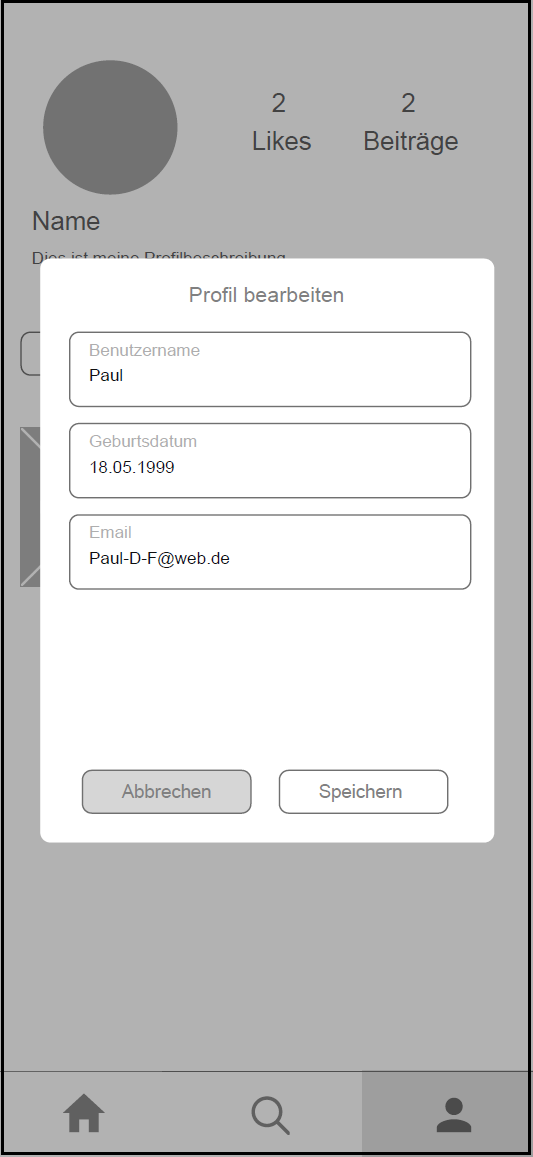
\includegraphics[width=.6\linewidth]{images/Edit_Profil_MockUp.png}
      \caption{Eigenes Profil bearbeiten}
      \label{fig:edit_profil}
    \end{minipage}
\end{figure}

Der Vorgang beim Hochladen eines neuen Feeds wird in \autoref{fig:popup_new_feed} und \autoref{fig:edit_new_feed} visualisiert. Der Benutzer hat die Möglichkeit das Foto entweder aus der eigenen Galerie auszuwählen oder mit der Kamera aufzunehmen. Noch während dem Hochladevorgang kann der Benutzer dem Feed eine Beschreibung und die GPS-Informationen für die Standortangabe hinzufügen.

\begin{figure}[H]
    \centering
    \begin{minipage}{.5\textwidth}
      \centering
      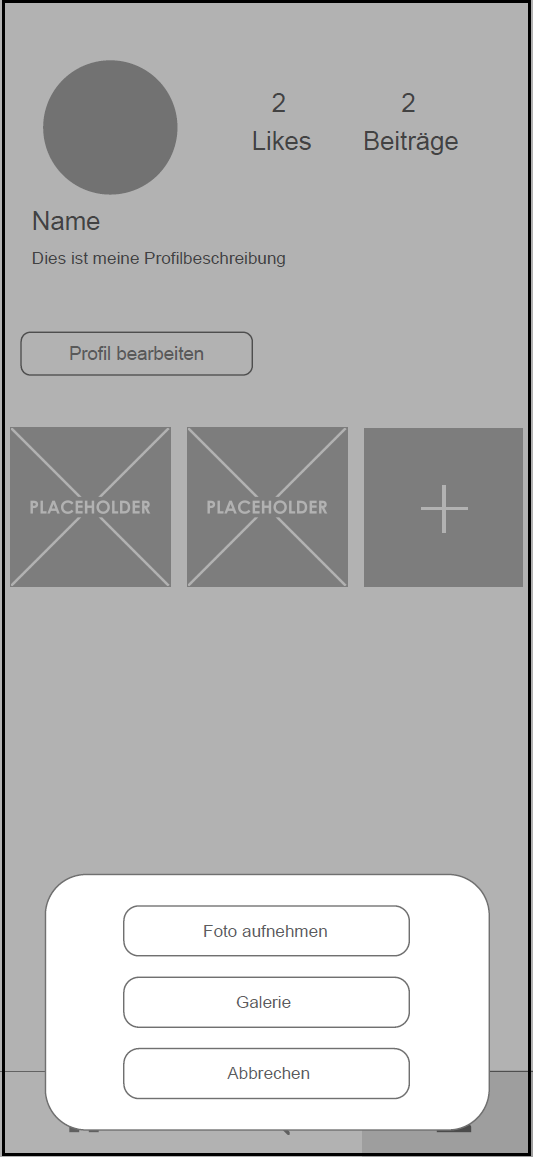
\includegraphics[width=.6\linewidth]{images/PopUp_Photo_MockUp.png}
      \caption{PopUp-Fenster für neuen Feed}
      \label{fig:popup_new_feed}
    \end{minipage}%
    \begin{minipage}{.5\textwidth}
      \centering
      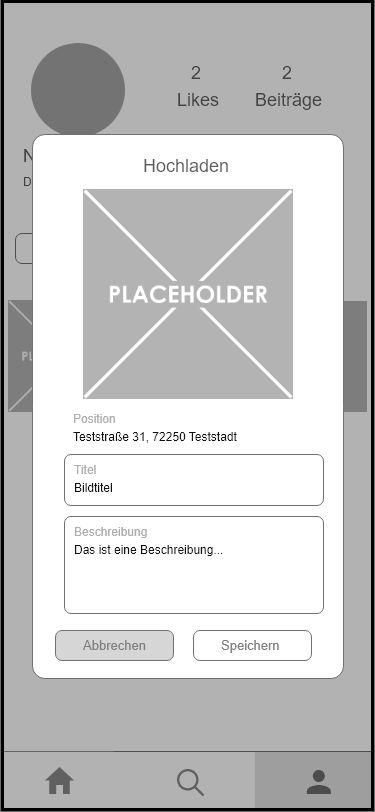
\includegraphics[width=.6\linewidth]{images/PopUp_Edit_New_Photo_MockUp.png}
      \caption{Neuen Feed bearbeiten}
      \label{fig:edit_new_feed}
    \end{minipage}
\end{figure}

\section{MVP-Kriterien\label{sec2.2:Unterpunkt-2}}

Folgende Kriterien müssen für eine erste, minimal funktionsfähige Iteration der mobilen Anwendung \glqq Geogram\grqq{}, während der Implementierung umgesetzt werden:

\begin{itemize}
    \item Login/Nutzerverwaltung
    \item Upload-Funktion für die Bilder mit Standortdaten
    \item Zugriff auf die Kamerafunktion des Mobilgerätes
    \item Zugriff auf die GPS-Daten (GPS-Modul des Mobilgerätes)
    \item Datenbank für Benutzerkonten, Standortdaten und Bildern
    \item Anzeigen der Beiträge
\end{itemize}

\section{Soll- und Kann-Kriterien\label{sec2.3:Unterpunkt-3}}

Neben den relevanten MVP-Kriterien wird die Konzeption noch mit Soll- und Kann-Kriterien ergänzt.

\textbf{Soll-Kriterien:}

\begin{itemize}
    \item Löschen von Bildern bzw. Beiträgen
    \item Hinzufügen von Bildbeschreibungen
    \item Ansicht des eigenen Kontos
    \item Einbindung von Google Maps für die Standortdaten
\end{itemize}

\textbf{Kann-Kriterien:}

\begin{itemize}
    \item Anmelden per Fingerabdruckssensor
    \item Anderen Benutzer \glqq folgen\grqq{} (\glqq folgen\grqq{}-Funktion)
    \item Benutzerdefinierte Filterfunktion für Beiträge
    \item Kommentare, Likes und Hastags für die Beiträge
    \item Dark-Mode abhängig von Systemeinstellungen
\end{itemize}
\chapter{Architektur\label{chap3:Drittes-Kapitel}}

Für die Architektur der mobilen Anwendung \glqq Geogram\grqq{}, wurden die zwei Frameworks \glqq Ionic\grqq{} und \glqq Express\grqq{} und die Entwicklungs-Plattform \glqq Firebase\grqq{} verwendet.

Wie in \autoref{fig:technologie} veranschaulicht, wird das Web-Framework \glqq Ionic\grqq{} für das Frontend verwendet. Das Backend kann in zwei Bereiche unterteilt werden. Zum einen wird die Entwicklungs-Plattform \glqq Firebase\grqq{} und das Node.js Web-Framework \glqq Express\grqq{} verwendet. Genauere Informationen bezüglich der Aufteilung des Backends wird in \autoref{sec3.2:Unterpunkt-2} beschrieben.

\begin{figure}[H]
    \centering
    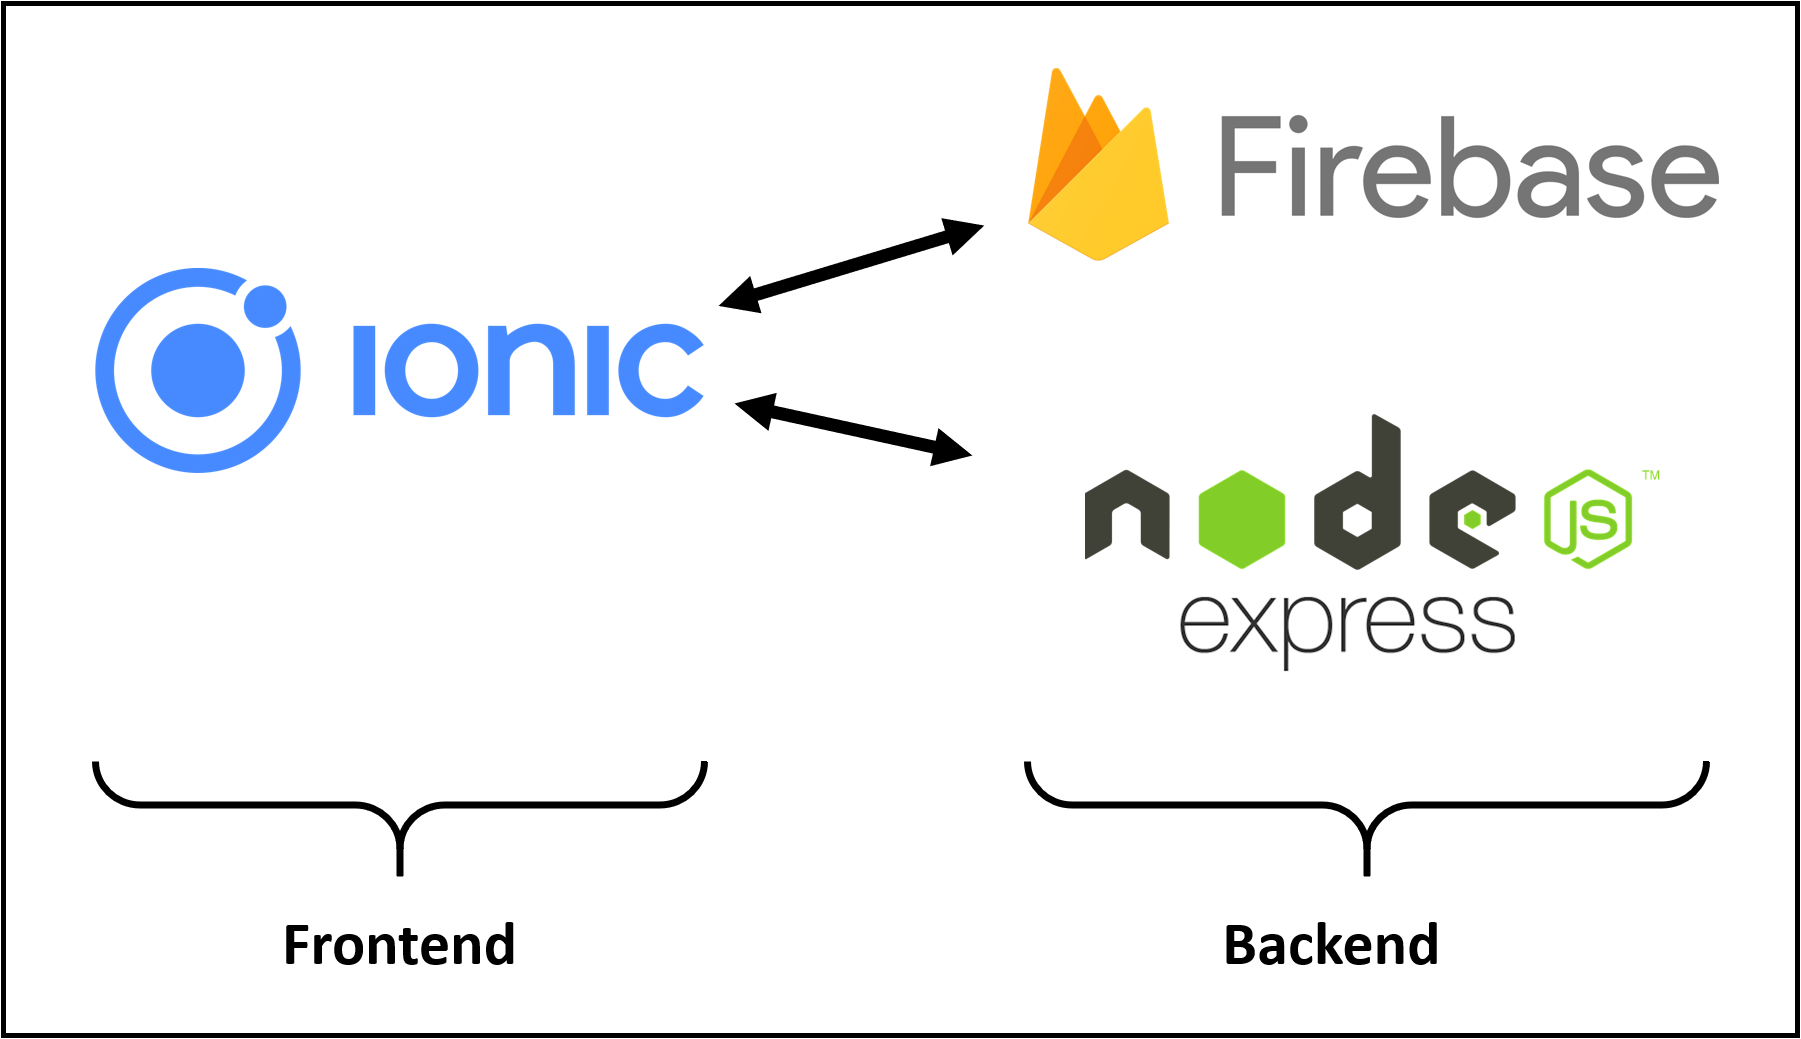
\includegraphics[width=.8\linewidth]{images/Architektur.png}
    \caption{Technologieübersicht}
    \label{fig:technologie}
\end{figure}

\section{Frontend\label{sec3.1:Unterpunkt-1}}

Inhalt

\section{Backend\label{sec3.2:Unterpunkt-2}}

Den Großteil der Backend-Aufgaben übernimmt die Entwicklungs-Platform Firebase. Verwendet wird hierfür die kostenlose \glqq Spark Plan\grqq{}-Version von Firebase. 

Die \textbf{Authentifizierung} und das \textbf{Credentialmanagent} wird hierbei vollständig von Firebase übernommen und verwaltet. Über vordefinierte Programmierschnittstellen kann man anschließend auf die Funktionen von Firebase zugreifen. Ebenso wird im kostenlosen Lizenzmodell \glqq Spark Plan\grqq{} eine Cloud-Speicherung namens \glqq \textbf{Firestore}\grqq{} angeboten. In der darin enthaltenen \textbf{Echtzeitdatenbank} stehen jedoch nur 1 GiB Speicherplatz zur Verfügung. Da sich das Kernkonzept von Geogram hauptsächlich um Fotos dreht und die finanziellen Mittel der Gruppe nicht für ein kostenpflichtiges Lizenzmodell ausreichen, wurde zusätzlich ein \textbf{Foto-Server} mithilfe des Web-Frameworks \glqq Express\grqq{} implementiert. Der Foto-Server wird von der Projekt-Gruppe selbst gehostet und beinhaltet mehr als 1 Gib Speicherplatz.

\subsection{Cloud Firestore\label{sup3.2.1:Unterpunkt-1}}

Die verwendete Firestore-Datenbank ist eine in der Cloud gehostete NoSQL-Datenbank. Über native SDKs können die iOS-, Android- und Web-Apps auf Firestore zugreifen.

\begin{wrapfigure}{r}{0.3\textwidth}
    \begin{center}
        
\includegraphics[width=0.3\textwidth]{images/firestore.png}
    \end{center}
    \caption{Speicherstruktur Firestore}
    \label{fig:storagestructure}
\end{wrapfigure}

In dem NoSQL-Datenmodell von Firestore, werden die Daten in Dokumente gespeichert, welche Felder enthalten, denen Werte zugeordnet sind. Diese Dokumente wiederrum werden in Sammlungen (collections) abgespeichert. Diese hierarchische Rangordnung der Datenspeicherung ist nochmals in \autoref{fig:storagestructure} abgebildet.

Für Geogram werden die zwei Sammlungen \glqq images\grqq{} und \glqq users\grqq{} benötigt. Wie die Bezeichnungen schon vermuten lassen, werden darin die Fotos und die Benutzer von Geogram abgespeichert.

Die Dokumente der Sammlung \glqq users\grqq{} bilden die verschiedenen Benutzerprofile von Geogram ab. Ein Benutzerprofil wird durch folgende Felder definiert:

\begin{itemize}
    \item \textbf{biography}: Eine kurze Beschreibung über den Benutzer
    \item \textbf{email}: Die E-Mail Adresse des Benutzers
    \item \textbf{profilepic}: URL zu dem Profilbild, welches im Foto-Server abgespeichert ist
    \item \textbf{userFirstName}: Vorname des Benutzers
    \item \textbf{userLastName}: Nachname des Benutzers
    \item \textbf{username}: Username des Benutzers
\end{itemize}

In \autoref{fig:users_collection} ist ein beispielhaftes users-Dokument abgebildet.

\begin{figure}[H]
    \centering
    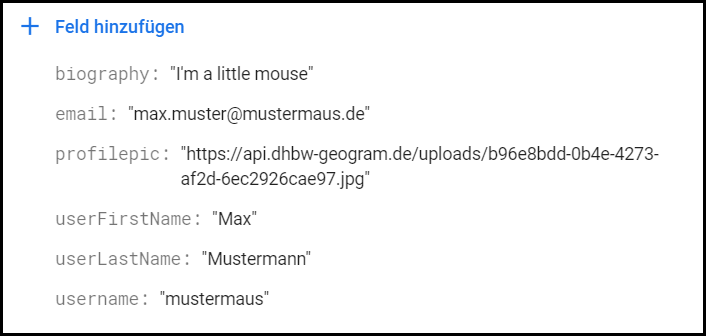
\includegraphics[width=.7\linewidth]{images/collection_users.png}
    \caption{Felder eines \glqq users\grqq{}-Dokumentes}
    \label{fig:users_collection}
\end{figure}

Die Dokumente der Sammlung \glqq images\grqq{} bilden die verschiedenen Bilder von Geogram ab. Ein Bild wird durch folgende Felder definiert:

\begin{itemize}
    \item \textbf{description}: Beschreibung des Bildes
    \item \textbf{id}: Eindeutige Id für das Bild
    \item \textbf{location}: GPS-Informationen für das Bild
    \item \textbf{timestamp}: Zeitpunkt des Hochladens des Bildes
    \item \textbf{title}: Titel des Bildes
    \item \textbf{url}: URL zu dem Bild, welches im Foto-Server abgespeichert ist
    \item \textbf{user}: Username des Bild-Inhabers
\end{itemize}

In \autoref{fig:images_collection} ist ein beispielhaftes images-Dokument abgebildet.

\begin{figure}[H]
    \centering
    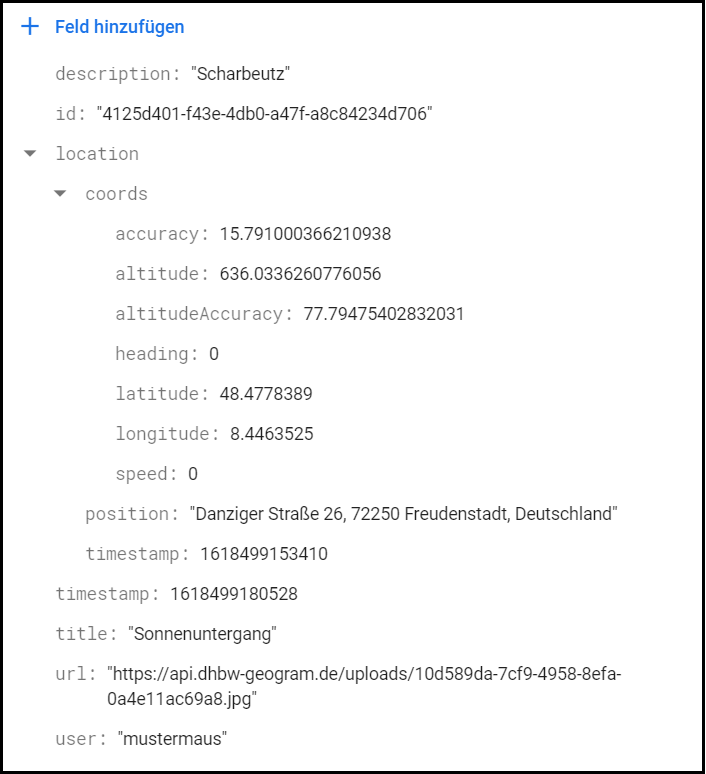
\includegraphics[width=.7\linewidth]{images/collection_images.png}
    \caption{Felder eines \glqq images\grqq{}-Dokumentes}
    \label{fig:images_collection}
\end{figure}

\subsection{Foto-Server\label{sup3.2.1:Unterpunkt-1}}

Text
\chapter{User-Guide\label{chap4:Viertes-Kapitel}}

Im folgenden Kapitel wird ein Überblick über alle implementierten Funktionalitäten aufgezeigt. So dient folgendes Kapitel auch als eine Art \glqq User-Guide\grqq{}.

\section{Login-/Logout-/Nutzerverwaltung\label{sec4.1:Unterpunkt-1}}

\begin{figure}[H]
    \centering
    \begin{minipage}{.4\textwidth}
        \begin{center}
            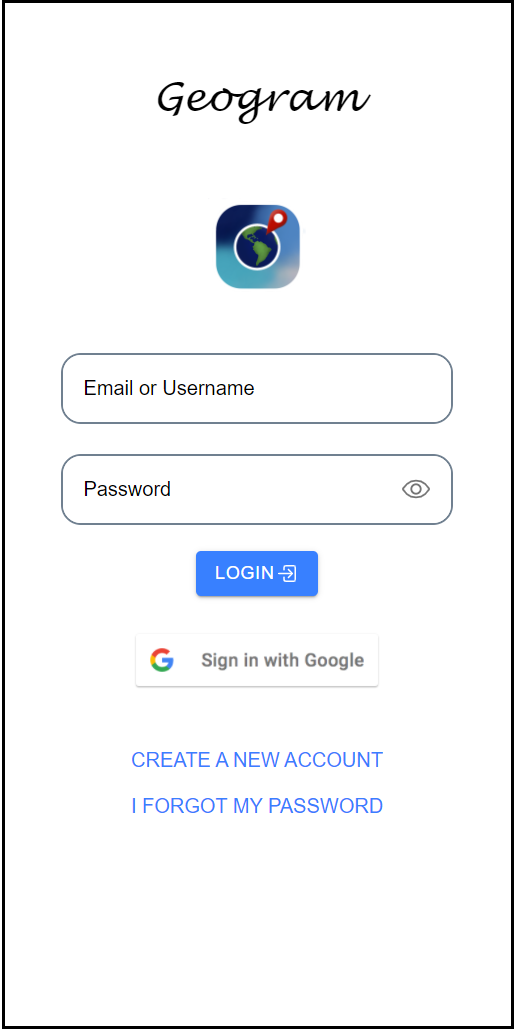
\includegraphics[width=0.8\linewidth]{images/Login.png}
        \end{center}
        \caption{Login - Ansicht}
        \label{fig:login}
    \end{minipage}%
    \begin{minipage}{.6\textwidth}
        \begin{changemargin}{0.5cm}{0cm}            
        Für den Anmeldevorgang benötigt der Besucher ein gültigen Account. Für die eigentliche Anmeldung wird das Passwort mit entweder der E-Mail-Adresse oder dem Usernamen benötigt. Zudem besteht auch die Möglichkeit sich mit einem Google-Account anzumelden.
        
        Sind die angegebenen Anmeldeinformationen nicht korrekt wird dem Besucher ein PopUp mit der Nachricht \glqq \textbf{Your Login credentials are incorrect}\grqq{} angezeigt.

        Neben dem Anmelden kann man über diese Ansicht noch die Funktionalitäten \glqq \textbf{Registrierung}\grqq{} und \glqq \textbf{Password vergessen}\grqq{} aufrufen.
        \end{changemargin}
    \end{minipage}
\end{figure}

\begin{figure}[H]
    \centering
    \begin{minipage}{.4\textwidth}
        \begin{center}
            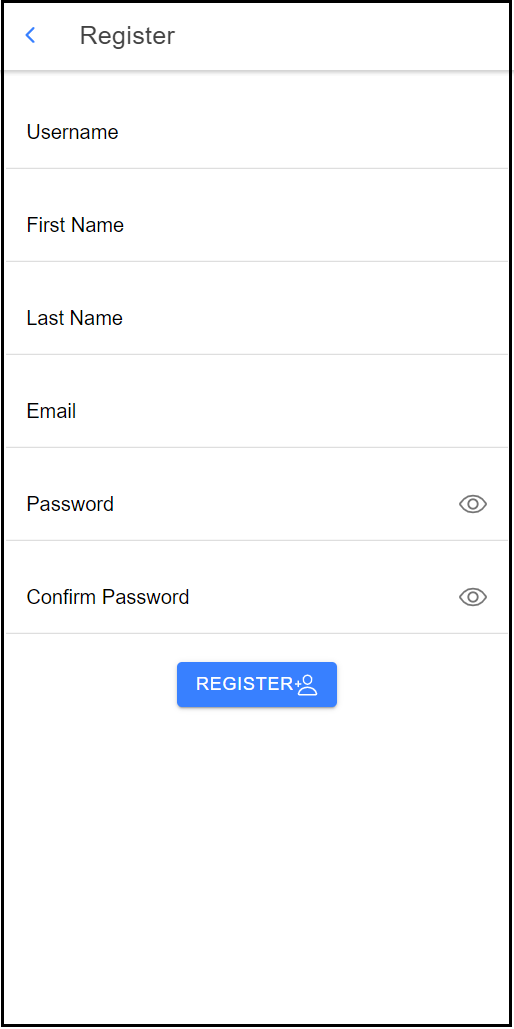
\includegraphics[width=0.8\linewidth]{images/Register.png}
        \end{center}
        \caption{Registrierungs - Ansicht}
        \label{fig:register}
    \end{minipage}%
    \begin{minipage}{.6\textwidth}
        \begin{changemargin}{0.5cm}{0cm}            
            Betätigt man auf der Login-Ansicht den Button \glqq \textbf{CREATE A NEW ACCOUNT}\grqq{}, so gelangt man auf die Registrierungs-Ansicht. Für einen neuen Account benötigt man folgende Informationen:

            \begin{itemize}
                \item \textbf{Username}
                \item \textbf{Vorname}
                \item \textbf{Nachname}
                \item \textbf{E-Mail}
                \item \textbf{Passwort}
            \end{itemize}

            Das Passwort muss folgende Bedingungen erfüllen:
            \begin{itemize}
                \item \textbf{Mindestens 6 Zeichen lang}
                \item \textbf{mind. eine Zahl}
                \item \textbf{mind. ein Sonderzeichen}
            \end{itemize}
        \end{changemargin}
    \end{minipage}
\end{figure}

\begin{figure}[H]
    \centering
    \begin{minipage}{.4\textwidth}
        \begin{center}
            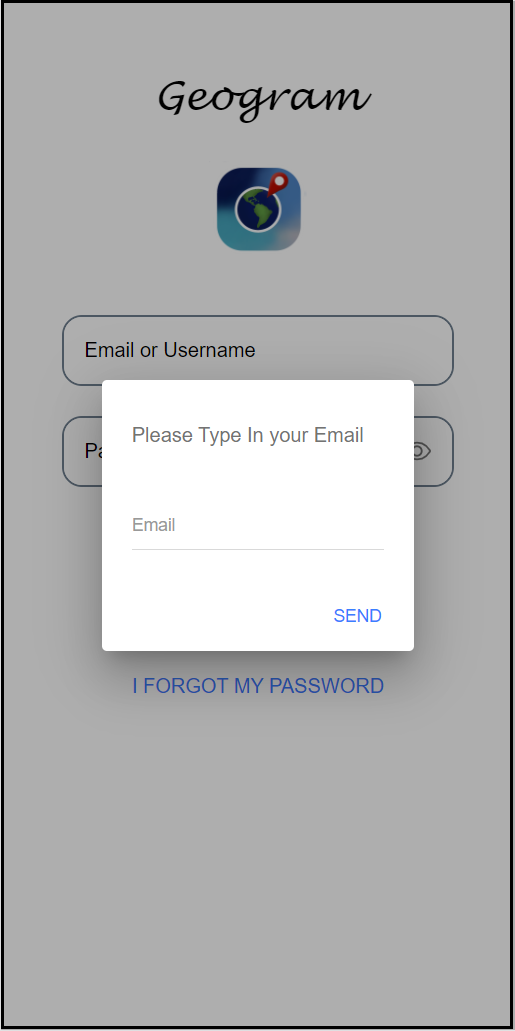
\includegraphics[width=0.8\linewidth]{images/forgetemail.png}
        \end{center}
        \caption{E-Mail-Vergessen - Ansicht}
        \label{fig:forgetemail}
    \end{minipage}%
    \begin{minipage}{.6\textwidth}
        \begin{changemargin}{0.5cm}{0cm}            
            Falls der Besucher sein Password für seinen Account vergessen hat, so kann er mit der \glqq Password-Vergessen\grqq{}-Funktionalität ein neues Password hinterlegen. Hierfür muss er seine gültige Account-E-Mail angeben und erhält von Geogram eine E-Mail zugesendet. In dieser E-Mail befindet sich ein Link, mit welchem der Besucher seinem Account ein neues Password hinterlegen kann.
        \end{changemargin}
    \end{minipage}
\end{figure}

\section{Profil - Ansicht\label{sec4.2:Unterpunkt-2}}

\begin{figure}[H]
    \centering
    \begin{minipage}{.4\textwidth}
        \begin{center}
            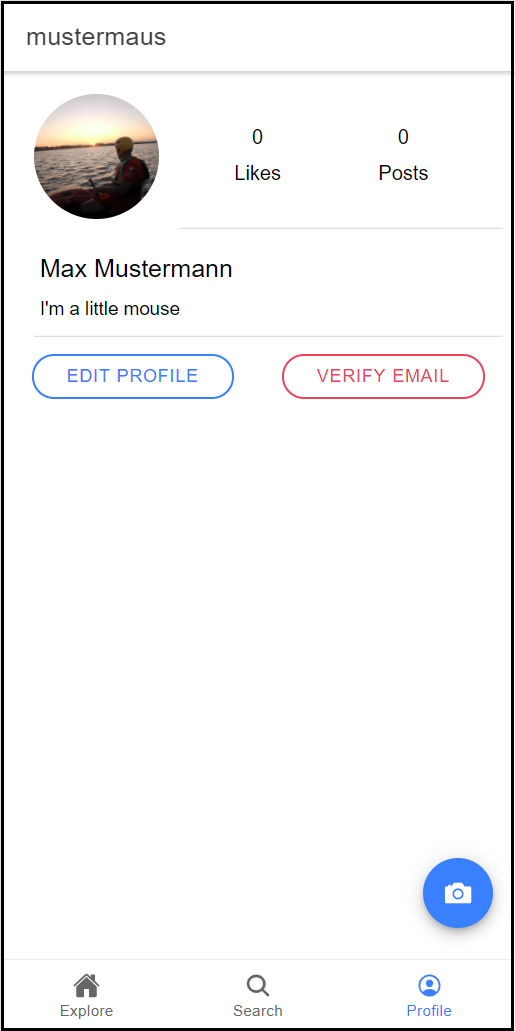
\includegraphics[width=0.8\linewidth]{images/profil.png}
        \end{center}
        \caption{Profil - Ansicht}
        \label{fig:profil}
    \end{minipage}%
    \begin{minipage}{.6\textwidth}
        \begin{changemargin}{0.5cm}{0cm}            
            In der Profil-Ansicht hat der Benutzer die Möglichkeit Informationen über sein eigenes Profil zu sehen.

            Zu sehen sind folgende Informationen:
            \begin{itemize}
                \item \textbf{Profilbild}
                \item \textbf{Anzahl erhaltener Likes}
                \item \textbf{Anzahl veröffentlichter Posts}
                \item \textbf{Vor- und Nachname}
                \item \textbf{Biographie (Text über sich selbst)}
                \item \textbf{Die eigenen Posts}
            \end{itemize}

            Zusätzlich hat man noch die Möglichkeit folgende Funktionalitäten auf der Profil-Ansicht auszuführen:
            \begin{itemize}
                \item \textbf{Ändern des Profilbildes (Durch drücken des Bildes)}
                \item \textbf{Profil bearbeiten}
                \item \textbf{Einmalige Verifizierung der E-Mail}
            \end{itemize}
        \end{changemargin}
    \end{minipage}
\end{figure}

Mit drücken eines Posts öffnet sich das PopUp aus \autoref{fig:post_popup}, über welches man auf die Post-Info aus \autoref{fig:post_info} gelangt.

\begin{figure}[H]
    \centering
    \begin{minipage}{.5\textwidth}
      \centering
      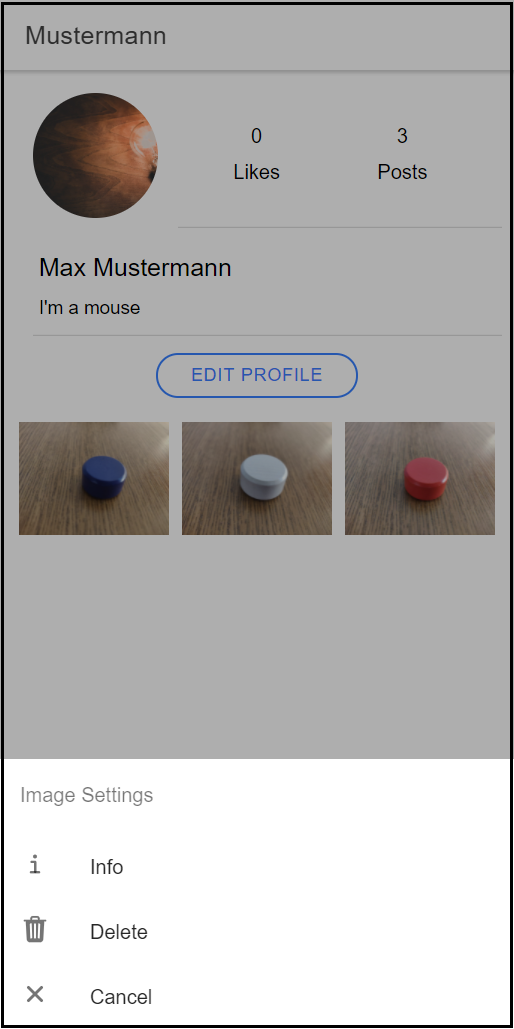
\includegraphics[width=.6\linewidth]{images/post_popup.png}
      \caption{Post-PopUp}
      \label{fig:post_popup}
    \end{minipage}%
    \begin{minipage}{.5\textwidth}
      \centering
      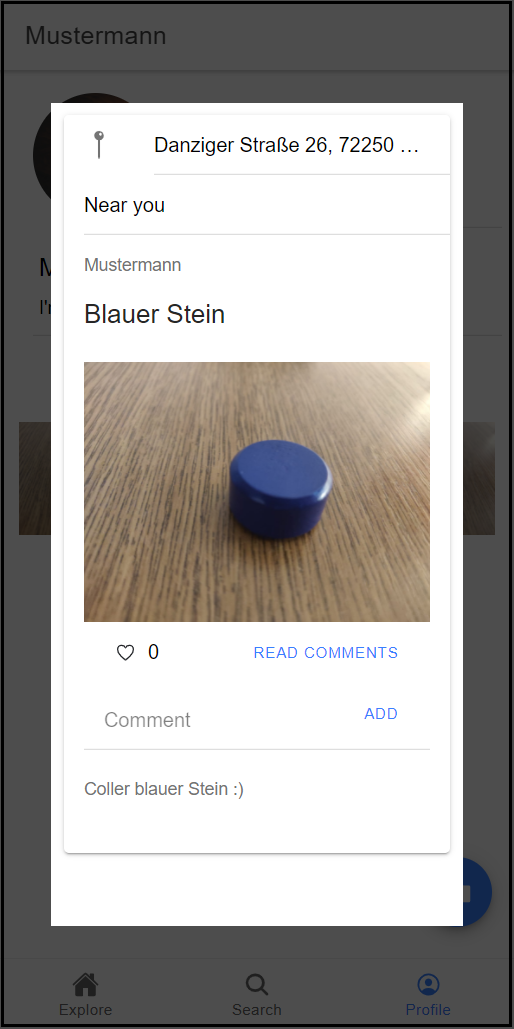
\includegraphics[width=.6\linewidth]{images/post_info.png}
      \caption{Post Informationen}
      \label{fig:post_info}
    \end{minipage}
\end{figure}

\begin{figure}[H]
    \centering
    \begin{minipage}{.4\textwidth}
        \begin{center}
            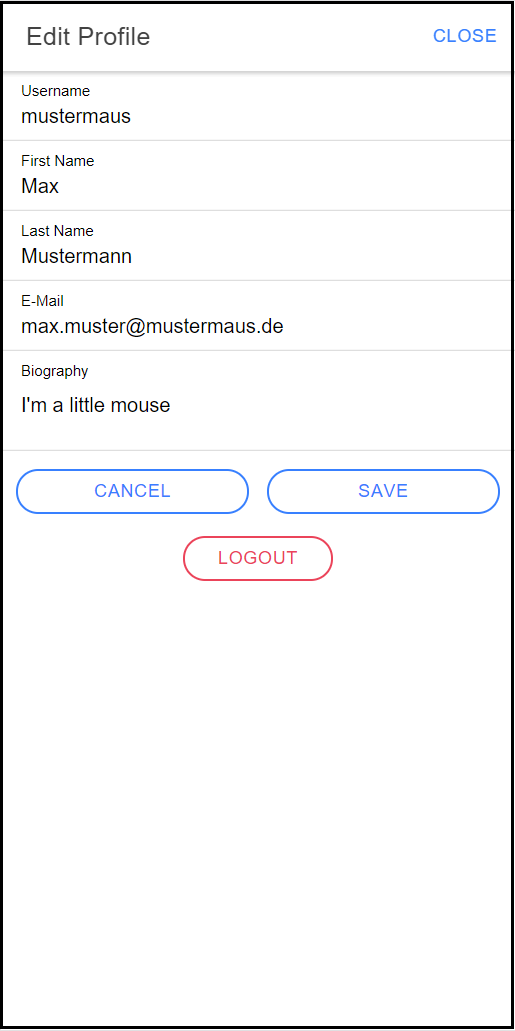
\includegraphics[width=0.8\linewidth]{images/editProfil.png}
        \end{center}
        \caption{Edit Profil - Ansicht}
        \label{fig:editprofil}
    \end{minipage}%
    \begin{minipage}{.6\textwidth}
        \begin{changemargin}{0.5cm}{0cm}            
            In dieser Ansicht hat der Benutzer zusätzlich die Möglichkeit die Informationen des Profils zu überarbeiten.

            Bearbeitet werden können folgende Informationen:
            \begin{itemize}
                \item \textbf{Benutzername}
                \item \textbf{Vorname}
                \item \textbf{Nachname}
                \item \textbf{E-Mail}
                \item \textbf{Biographie (Text über sich selbst)}
            \end{itemize}

            Zusätzlich hat man hier die Möglichkeit sich von Geogram abzumelden. Man gelangt dann wieder zur Login-Ansicht.
        \end{changemargin}
    \end{minipage}
\end{figure}

\section{Suchen - Ansicht\label{sec4.3:Unterpunkt-3}}

\begin{figure}[H]
    \centering
    \begin{minipage}{.4\textwidth}
        \begin{center}
            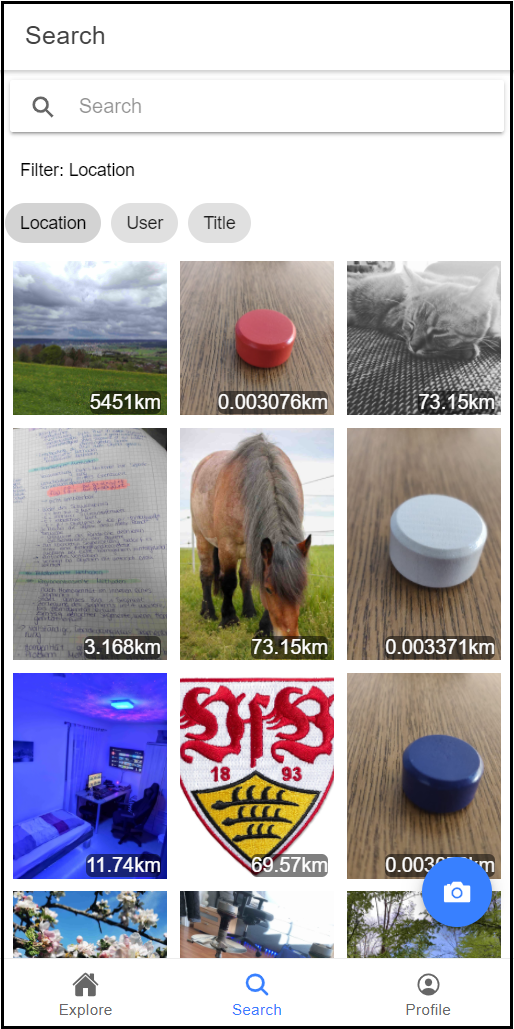
\includegraphics[width=0.8\linewidth]{images/Search.png}
        \end{center}
        \caption{Suchen - Ansicht}
        \label{fig:searchTab}
    \end{minipage}%
    \begin{minipage}{.6\textwidth}
        \begin{changemargin}{0.5cm}{0cm}            
            Mit dem Tab \glqq \textbf{Search}\grqq{} gelangt der Benutzer auf die nebenstehende Ansicht. Hier hat der Benutzer die Möglichkeit nach bestimmten Posts zu suchen.

            Bei den einzelnen Posts werden jeweils die Bilder und die dazugehörigen Entfernungen zum Benutzer angezeigt und erst beim Drücken eines Posts erhält man eine Info-Ansicht, wie aus \autoref{fig:post_info}.

            Zu Beginn werden alle verfügbaren Posts angezeigt. Der Benutzer hat jedoch auch die Möglichkeit die angezeigten Posts zu filtern. Gefiltert werden kann nach der Entfernung, dem User oder dem Titel.
        \end{changemargin}
    \end{minipage}
\end{figure}

\section{Explore - Ansicht\label{sec4.4:Unterpunkt-4}}

\begin{figure}[H]
    \centering
    \begin{minipage}{.4\textwidth}
        \begin{center}
            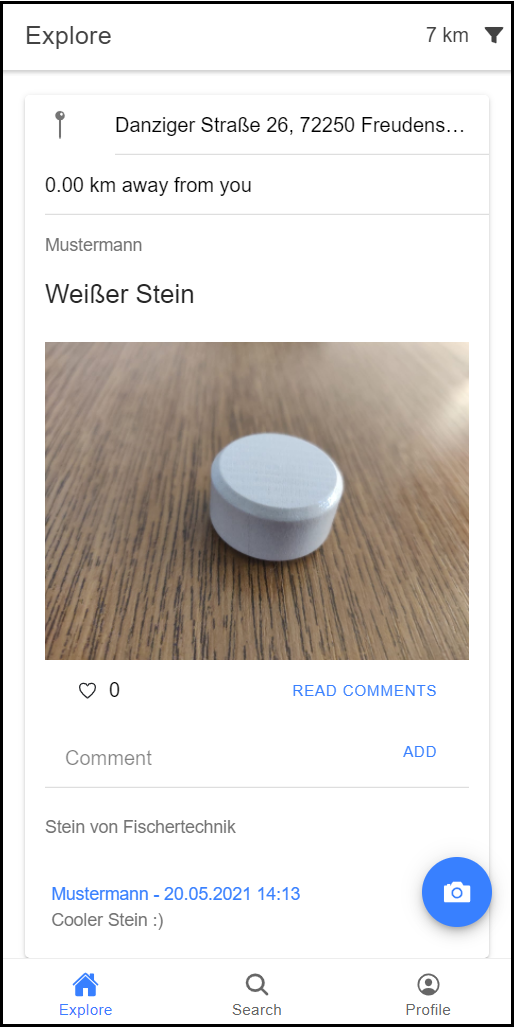
\includegraphics[width=0.8\linewidth]{images/explore.png}
        \end{center}
        \caption{Explore - Ansicht}
        \label{fig:exploreTab}
    \end{minipage}%
    \begin{minipage}{.6\textwidth}
        \begin{changemargin}{0.5cm}{0cm}            
            Mit dem Tab \glqq \textbf{Explore}\grqq{} gelangt der Benutzer auf die nebenstehende Ansicht. Hier werden dem Benutzer die vollständigen Posts angezeigt.

            Dem Benutzer werden die Posts abhängig von der Entfernung entweder angezeigt oder nicht. Um den Radius der Entfernung zu ändern, kann der Benutzer diesen oben rechts einstellen. Wird der Radius auf \glqq \textbf{30+}\grqq{} gestellt, so werden alle Posts angezeigt.

            Bei jedem Post hat der Benutzer die Möglichkeit ein Like und Kommentare abzugeben. Den eigenen Kommentar und die Kommentare von anderen Benutzern kann man ebenfalls unter den Posts sehen. 
        \end{changemargin}
    \end{minipage}
\end{figure}

\end{document}